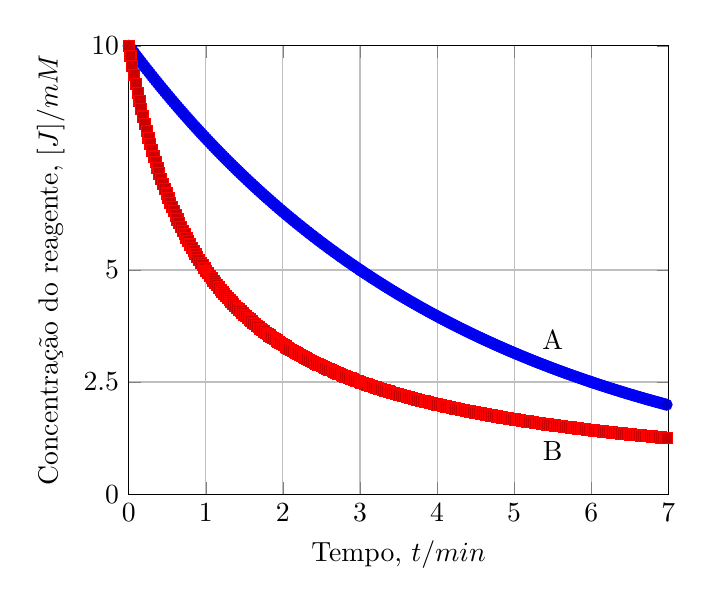
\begin{tikzpicture}
    \begin{axis}
        [
            xlabel = {Tempo, $t/\unit{min}$},
            ylabel = {Concentração do reagente, $[\ce{J}]/\unit{mM}$},
            ymin = 0, ymax = 10,
            xmin = 0, xmax = 7,
            domain = 0:7,
            grid = major,
            samples = 300,
            ytick = {0, 2.5, 5, 10},
        ]

    \addplot+ [ blue ]
        {
            10*2^(-x/3)
        };

    \addplot+ [ red ]
        {
            1/(1/10 + x/10)
        };
        
    \addplot [ mark=*, color=blue, only marks ] coordinates
        { 
            (3, 5) 
            (6, 2.5) 
        };

    \addplot [ mark=*, color=red, only marks ] coordinates
        { 
            (1, 5) 
            (3, 2.5) 
        };
    
    \node [anchor = south] at (axis cs:5.5, 3) 
        { \ce{A} };
        
    \node [anchor = north] at (axis cs:5.5, 1.4) 
        { \ce{B} };

    \end{axis}
\end{tikzpicture}